%% Generic single-column journal submission template (article class)
%% Compatible with Elsevier / Springer / Wiley / arXiv / IEEE Access
%% Wide-Scale Sampling with Hard-Argmin Selection and CBF Projection
\documentclass[11pt,onecolumn,a4paper]{article}

\usepackage[margin=1in]{geometry}
\usepackage{amsmath,amssymb,amsfonts,amsthm}
\usepackage{graphicx}
\usepackage{booktabs}
\usepackage{multirow}
\usepackage{array}
\usepackage[noend]{algpseudocode}
\usepackage{algorithm}
\usepackage{cite}
\usepackage{url}
\usepackage{authblk}
\usepackage{lineno}
\usepackage{caption}
\usepackage{titlesec}
\usepackage{xcolor}
\usepackage[toc,page]{appendix}
\usepackage{hyperref}
\hypersetup{colorlinks=true,linkcolor=black,citecolor=black,urlcolor=black}

% Line numbers for peer review
\linenumbers
\renewcommand{\linenumberfont}{\normalfont\scriptsize\sffamily\color{gray}}

% Section heading style (numbered Section 1, 1.1, 1.1.1)
\titleformat{\section}{\normalfont\Large\bfseries}{\thesection.}{0.6em}{}
\titleformat{\subsection}{\normalfont\large\bfseries}{\thesubsection}{0.6em}{}
\titleformat{\subsubsection}{\normalfont\normalsize\bfseries}{\thesubsubsection}{0.6em}{}

% Caption style
\captionsetup{labelfont=bf,font=small,labelsep=period}

% Allow wider line breaking tolerance to suppress Overfull \hbox on
% paragraphs with long \texttt{} identifiers and URLs
\sloppy
\tolerance=2000
\emergencystretch=10pt

\newtheorem{proposition}{Proposition}
\newtheorem{remark}{Remark}

% Shorthand
\newcommand{\R}{\mathbb{R}}
\newcommand{\E}{\mathbb{E}}
\newcommand{\Nm}{N_{\mathrm{MC}}}
\newcommand{\spt}{\mathrm{sp}}
\newcommand{\pd}{\mathrm{pd}}
\newcommand{\dt}{\Delta t}
\newcommand{\nom}{\mathrm{nom}}
\newcommand{\safe}{\mathrm{safe}}
\newcommand{\TErr}{\mathrm{TErr}}
\newcommand{\IAE}{\mathrm{IAE}}

\begin{document}

\title{\textbf{WIDE-SCALE SAMPLING WITH HARD-ARGMIN SELECTION AND CBF PROJECTION
FOR SAFE QUADROTOR NAVIGATION IN NARROW PASSAGES}}

% Authors removed for double-blind review.
% See cover page for author names, affiliations, and contact information.

\date{}
\maketitle

\begin{abstract}\noindent
A common implementation of sampling-based NMPC for quadrotor obstacle
avoidance draws candidate commands from a narrow Gaussian around a PD
nominal. In tight passages, this nominal can point toward the
conservative composite-barrier boundary rather than through the actual
geometric gap. Adding more samples close to that nominal does not
address this failure mode --- it is a candidate-generation problem,
not a solver problem. TSH-NMPC widens the sampling distribution
($\sigma = 5\,\mathrm{N}$ around the PD nominal at $K = 10$),
selects the lowest-cost rollout by hard argmin, and projects the
result through a DT-CBF quadratic program before execution. On the
narrow-passage benchmark, the wide-scale sampler reached 97--99\%
success, while the narrow-scale PD-Gaussian baseline reached
64--70\%. Under $+50\%$ mass mismatch the baseline failed in all
40 trials; the wide-scale variants retained 77.5\%--82.5\% success.
Compared with CasADi+IPOPT, TSH-NMPC achieved the same success rate
at roughly 6 ms per call with a fixed $O(K \cdot S)$ rollout budget,
although CasADi retained lower terminal error. A learned-proposal
ablation reduced success from 97.7\% to 88.7\%, suggesting that
coverage mattered more than prediction accuracy in this setting.
\end{abstract}

\medskip
\noindent\textbf{Key Words:} Nonlinear model predictive control; sampling-based MPC; control barrier functions; quadrotor obstacle avoidance.
\medskip

%====================================================================
\section{Introduction}
%====================================================================

When flying a quadrotor and needing to avoid obstacles, the controller
has to handle non-convex collision rules fast, on a small chip inside
the drone. Sampling-based NMPC is quite good for this because it just
rolls out different candidate controls through a model, and you do
not need convexity or differentiability of the cost. The per-step work
is bounded ($K$ rollouts of $S$ steps each) and easy to run in
parallel. Two common versions that people use are MPPI
\cite{WIL17,WIL18} and CEM \cite{BOT13}.

The usual \emph{single-source} setup draws all $K$ first-step
candidates from one Gaussian around a nominal control. When the
nominal points at an obstacle boundary --- as often happens in narrow
passages, where the conservative composite barrier treats a
geometrically feasible gap as unsafe --- every candidate picks up the
same directional bias. Making $K$ larger inside a narrow sampling
scale does not fix this: more samples near a bad nominal stay near
that nominal. On our narrow-passage benchmark, single-source
PD-Gaussian rollout NMPC reached only $73.8\%$ success at $K = 20$
(Section~\ref{sec:exp-main}). The pattern suggests that what matters
is not just how many candidates you draw, but where you draw them
from.

The useful change was not just to draw from a wider Gaussian. Wider
sampling can produce controls that point through the geometric gap,
but it also produces unsafe commands that need filtering. Hard
selection matters because the useful escape candidates are sparse
inside the pool, and soft aggregation can wash them out. Safety
projection matters because some of the wider samples land outside
the safe set. In the experiments below, the three changes played separable empirical
roles (Fig.~\ref{fig:mechanism}). \textbf{(P1)}~Wider sampling
($\sigma = 5\,\mathrm{N}$ per axis) raised the odds of drawing an
escape candidate. \textbf{(P2)}~Hard argmin kept sparse escape
candidates. \textbf{(P3)}~DT-CBF projection filtered the unsafe
subset of the wider pool. Taking away any one changed a different
piece of the failure mode.

\begin{figure}[t]
\centering
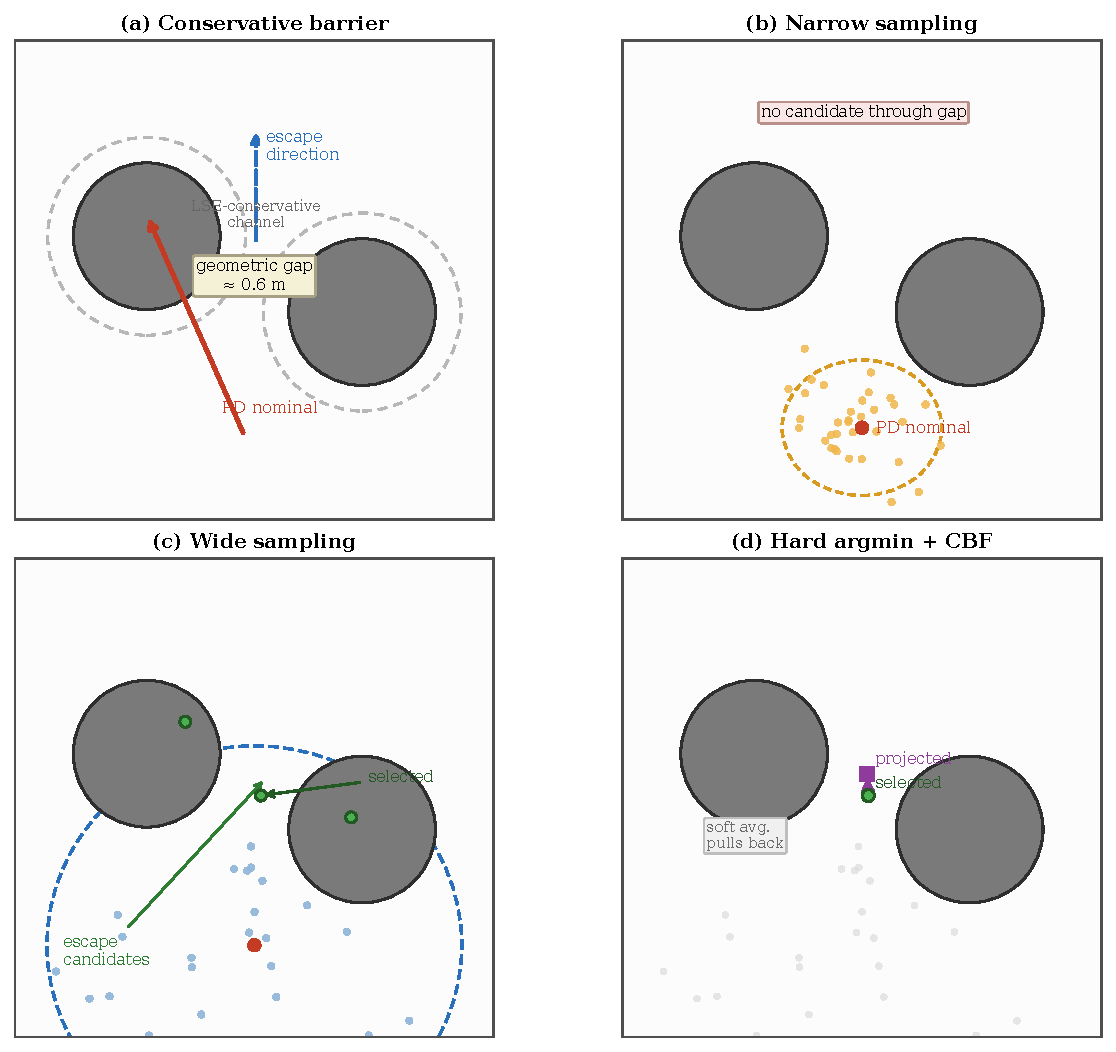
\includegraphics[width=\textwidth]{experiments/results_v6/fig1_mechanism.pdf}
\caption{Candidate-generation failure and the three roles of
TSH-NMPC. Narrow PD-centred sampling can miss the escape direction,
while wide sampling creates sparse escape candidates. Hard argmin
preserves the selected escape, and DT-CBF projection filters it
before execution.}
\label{fig:mechanism}
\end{figure}

\subsection{Contributions}

\begin{enumerate}
\item \textbf{Mechanistic diagnosis and controller design.}
Single-source PD-Gaussian sampling fails in narrow passages because
the candidate pool inherits the directional bias of the nominal.
TSH-NMPC couples wide sampling, hard-argmin selection, and DT-CBF
projection to address escape generation, candidate preservation, and
collision safety, respectively.

\item \textbf{Empirical decomposition.} The ablations show that
narrowing the sampling scale caps success, soft selection degrades
terminal tracking, and removing the CBF projection causes collisions.
These effects support the view that the three design choices act on
different parts of the narrow-passage failure mode.

\item \textbf{Controlled comparisons.} A learned-prior ablation shows
that candidate-space coverage can dominate single-candidate prediction
accuracy in this benchmark. Compared with CasADi+IPOPT, TSH-NMPC
provides solver-free, fixed-budget computation rather than higher
terminal accuracy.
\end{enumerate}

\subsection{Related Work}

\textbf{Sampling NMPC.} MPPI \cite{WIL17,WIL18} uses
importance-weighted averaging of $K$ Gaussian-perturbed trajectories.
This works well when many candidates provide graded improvement, but
can dilute sparse escape directions in tight passages
\cite{SUN22,GAN21}. CEM \cite{BOT13,RUB04} iteratively refits the
proposal to the top-$\beta$ quantile, at the cost of additional
rollout evaluations. TSH-NMPC uses a fixed wide scale and hard
selection without refitting or averaging.

\textbf{CBFs, learned proposals, and scenario optimisation.}
Continuous-time CBFs \cite{AME17} enforce forward-invariance;
discrete-time variants \cite{WAN17} extend this to sampled-data
execution. This paper uses DT-CCBF as a safety filter for wide
exploration, not as a new CBF. Prior works replace the Gaussian
proposal by a learned distribution \cite{PAN17,KAH18,OKA20,JAN22},
but few compare against an isotropic random source at matched budget
(Section~\ref{sec:exp-negabl}). Scenario optimisation
\cite{CAM08,CAM18} bounds violation probability under a convexity
assumption. TSH-NMPC satisfies only the weaker monotone property
(Proposition~\ref{prop:mono}) and makes no violation-probability
claim.

%====================================================================
\section{Problem Formulation and Background}\label{sec:problem}
%====================================================================

\subsection{Quadrotor Abstract Translational Dynamics}

The outer-loop translational guidance operates on a 6D state
$x_t = [p_t^\top, v_t^\top]^\top \in \R^6$. The virtual control
$u_t \in \R^3$ is the gravity-precompensated net force command; the
inner-loop attitude controller is assumed fast enough
($T_{\mathrm{att}} \ll \dt$) that flatness-mapped tracking does not
affect the translational closed loop. Discrete-time dynamics:
\begin{equation}\label{eq:dyn}
x_{t+1} = A_d x_t + B_d u_t,\quad
A_d = \begin{pmatrix} I_3 & \dt\, I_3 \\ 0 & I_3 \end{pmatrix},\;
B_d = \tfrac{\dt}{m} \begin{pmatrix} 0 \\ I_3 \end{pmatrix},
\end{equation}
with body drag omitted in the nominal model (added in simulation,
Section~\ref{sec:exp-setup}). Input saturation:
$u_t \in [u_{\min}, u_{\max}]^3$, $u_{\max} = 15\,\mathrm{N}$.

\subsection{Discrete-Time Composite CBF (DT-CCBF)}

Let $\mathcal{C}_i = \{x \in \R^6 : h_i(x) \ge 0\}$ be the
obstacle-free set for obstacle $i$, with $h_i(x) = \|p - p_i\|^2 - r_i^2$.
The unsafe set $\cup_i \overline{\mathcal{C}}_i$ is non-convex. We
replace the per-obstacle minimum by the LSE composite:
\begin{equation}\label{eq:lse}
h(x) = -\tfrac{1}{\kappa} \log \sum_{i=1}^{M}
\exp\!\big(-\kappa\, h_i(x)\big), \quad \kappa = 5,
\end{equation}
with $h(x) \le \min_i h_i(x)$ and $h(x) \to \min_i h_i(x)$ as
$\kappa \to \infty$.

\emph{Remark (LSE conservatism).}
For $M = 5$ and $\kappa = 5$, the LSE composite introduces a
conservative barrier-value offset of $\kappa^{-1}\log M \approx
0.32$\,m$^2$. Because $h_i$ is quadratic in distance, this offset
should not be interpreted as a constant radial inflation; locally
it corresponds to an equivalent radial shift $\Delta r \approx
\sqrt{r^2 + \kappa^{-1}\log M} - r$, which reduces the apparent
passage width. On \textsc{narrow}, the geometric gap is
${\approx}0.6\,\mathrm{m}$, so the LSE-conservative channel is
substantially narrower.
The DT-CBF condition \cite{WAN17,AME17}:
\begin{equation}\label{eq:dt-ccbf}
h(x_{t+1}) \ge (1 - \alpha_d)\, h(x_t) - \gamma_d
\end{equation}
with $(\alpha_d, \gamma_d) = (0.8, 0.2)$. Linearising about
\eqref{eq:dyn} yields $A(x_t)^\top u \le b(x_t)$. The safety filter:
\begin{equation}\label{eq:qp}
u_\safe = \operatorname*{arg\,min}_{u \in [u_{\min}, u_{\max}]^3}
\tfrac{1}{2} \|u - u_\nom\|^2
\quad \text{s.t.}\; A(x_t)^\top u \le b(x_t)
\end{equation}
projects $u_\nom$ onto the safe set. When infeasible, a box-constrained
fallback with $\delta_{\mathrm{buffer}} = 0.15\,\mathrm{m}$ is used.

\subsection{Sampling NMPC}

Given $x_t$, $x_\spt$, and budget $K$, a sampling NMPC controller
builds $K$ first-step candidates $\{u^{(k)}\}_{k=1}^{K}$, scores each
by simulation-based cost $J^{(k)}$, and executes the lowest-cost
candidate after CBF projection. The formulation is
\emph{single-source} when all $K$ candidates share one Gaussian:
\begin{equation}\label{eq:single}
u^{(k)} \sim \mathcal{N}(\mu_t, \sigma^2 I_3),\quad k = 1,\dots,K,
\end{equation}
centred at a single nominal $\mu_t$. MPPI \cite{WIL17} replaces hard
argmin by importance-weighted averaging; CEM \cite{BOT13} iteratively
refits a single-source Gaussian to the top-$\beta$ quantile.
\emph{Two-source} (Section~\ref{sec:method}) combines two Gaussians of
different covariances at the same nominal.

%====================================================================
\section{Method: Wide-Scale Sampling with Hard-Argmin Selection and CBF Projection}\label{sec:method}
%====================================================================

This section presents TSH-NMPC: $K$ candidates from a wide-scale
PD-centred Gaussian, scored by short rollout, hard-argmin selected,
and CBF-projected. No learned predictor, importance weighting, or
iterative refit is used (a learned-prior ablation appears in
Section~\ref{sec:exp-negabl}).

\subsection{Wide-Scale PD-Centred Candidate Generation}

At each step $t$, the controller draws $K$ first-step controls from a
wide-scale PD-centred Gaussian.

\textbf{Default: single-source-wide ($R_{0,\sigma=5}$).} With
$u_\pd(x_t, x_\spt) = m (K_p (p_\spt - p_t) + K_d (v_\spt - v_t))$,
$(K_p, K_d) = (4, 3)$:
\begin{equation}\label{eq:srcA}
u^{(k)} \sim \mathcal{N}(u_\pd, \sigma_r^2 I_3),\quad k = 1, \ldots, K,
\end{equation}
where $\sigma_r = 5.0\,\mathrm{N}$ is a fixed scalar (operating plateau
$[5, 8]$, Section~\ref{sec:exp-sigma-sweep}). At
$\sigma_r \approx u_{\max}/3$, the distribution escapes PD basins
while remaining narrow enough for rollout selection.

A two-source variant ($R_{1,\sigma=5}$) splits the budget evenly
between $\sigma_\pd = 2$ and $\sigma_r = 5$ and is empirically
equivalent to the single-source-wide form ($p = 0.51$,
Section~\ref{sec:exp-r0-pd-s5}).
All candidates are clamped:
\begin{equation}\label{eq:clip}
u^{(k)} \leftarrow \operatorname{clip}(u^{(k)}, u_{\min}, u_{\max}),
\quad k = 1, \ldots, K.
\end{equation}

\subsection{Rollout-Based First-Step Cost Evaluation}

Each candidate is scored by a short closed-loop rollout: $u^{(k)}$ at
$s=0$, PD baseline at $s=1,\dots,S-1$:
\begin{equation}\label{eq:rollout}
\tilde{u}_s^{(k)} =
\begin{cases}
u^{(k)}, & s = 0, \\
u_\pd(\tilde{x}_s^{(k)}, x_\spt), & 1 \le s \le S-1,
\end{cases}
\end{equation}
with $\tilde{x}_{s+1}^{(k)} = f(\tilde{x}_s^{(k)}, \tilde{u}_s^{(k)})$
(Section~\ref{sec:problem}), $S = 20$ ($0.4\,\mathrm{s}$). The cost is quadratic
with obstacle penalty:
\begin{equation}\label{eq:cost}
J^{(k)} = \sum_{s=1}^{S}\!\!\left(\!\|\tilde{x}_s^{(k)} - x_\spt\|_Q^2
+ R\,\|\tilde{u}_s^{(k)}\|^2
+ \rho \sum_i [\delta - d_i(\tilde{x}_s^{(k)})]_+^2\!\right),
\end{equation}
$Q = \operatorname{diag}(15,15,15,1,1,1)$, $R = 0.02$, $\rho = 2000$,
$\delta = 0.3\,\mathrm{m}$, $d_i(x) = \|p - p_i\| - r_i$. Hard-argmin:
\begin{equation}\label{eq:argmin}
k^\star = \operatorname*{arg\,min}_{1 \le k \le K} J^{(k)},
\quad u_\nom = u^{(k^\star)}.
\end{equation}
Rollout evaluation replaces Q-head pre-screening and MPPI averaging;
Proposition~\ref{prop:mono} gives the monotone $K$-cost relation.

\subsection{DT-CCBF Safety Projection}

$u_\nom$ from \eqref{eq:argmin} is projected onto the safe set via
the QP \eqref{eq:qp}, solved in closed form via active-set on $\R^3$.
The resulting $u_\safe$ is executed.

\subsection{Algorithm}

The closed-loop step is: compute the PD nominal, sample $K$ wide
candidates, clamp to actuator bounds, roll out each candidate for $S$
steps under the PD baseline, select the lowest-cost first input
(hard argmin), and project it through the DT-CBF QP. Unless stated
otherwise, all experiments use $K = 10$, $\sigma_r = 5\,\mathrm{N}$, $S = 20$,
$\kappa = 5$, with $\sigma_\pd = 2\,\mathrm{N}$ used only in the legacy
two-source variant.
\phantomsection\label{alg:tsh}

%====================================================================
\section{Theoretical Properties}\label{sec:theory}
%====================================================================

We record two properties. The theory is minimal: TSH-NMPC is a
sampling scheme atop an off-the-shelf DT-CCBF. We claim no stability
or convergence beyond what either component provides.

\subsection{Forward-Invariance of the Safe Set}

Since $h_i$ depends on position and the input enters through acceleration,
the input has relative degree~2 w.r.t.\ $h_i$. Expanding $h(x_{t+1})$
yields $A(x_t)^\top u \le b(x_t)$, with $A$, $b$ depending on the
barrier gradient, velocity, and $(\alpha_d, \gamma_d)$
(\cite[Thm.~1]{WAN17}, \cite[\S IV]{AME17}). The LSE composite
has $h(x) \le \min_i h_i(x)$, gap $\le \kappa^{-1}\log M \approx
0.32\,\mathrm{m}$; $h(x) \ge 0$ implies all per-obstacle barriers are
non-negative.

\begin{proposition}[Conditional DT-CBF invariance and empirical collision avoidance]
\label{prop:safety}
Let $\tilde h(x) := h(x) + \gamma_d/\alpha_d$,
$\tilde{\mathcal C} := \{x : \tilde h(x) \ge 0\}$.
\emph{Conditional on QP \eqref{eq:qp} feasibility at every step,}
$\tilde{\mathcal C}$ is forward invariant:
$x_t \in \tilde{\mathcal C} \Rightarrow x_{t+1} \in \tilde{\mathcal C}$.
The trajectory remains in $\{x : h(x) \ge -\gamma_d/\alpha_d\}$
(margin $= 0.25\,\mathrm{m}$).
\end{proposition}

If the QP has no feasible solution, a box-constrained fallback applies full
effort in the barrier-gradient direction. The proposition does not
apply during fallback, but $\delta_{\mathrm{buffer}} = 0.15\,\mathrm{m}$
absorbs the one-step excursion (${\approx}0.06\,\mathrm{m}$ at $v \le 3\,\mathrm{m}$/s).
Empirically, zero collisions are observed across all CBF-enabled
trials (Section~\ref{sec:exp-fallback}).

\subsection{Monotone Expected Min-Cost in $K$}

\begin{proposition}[Monotone expected cost]\label{prop:mono}
Let $u^{(1)},\dots,u^{(K)}$ be drawn independently from the sampling
distribution, then clamped to $[u_{\min}, u_{\max}]^3$.
Define $J^\star_K := \min_{1 \le k \le K} J(u^{(k)})$ where
$J(\cdot)$ is the rollout cost \eqref{eq:cost}. Then
$\E[J^\star_{K+1}] \le \E[J^\star_K]$ for every $K \ge 1$.
\end{proposition}

This is the non-convex analogue of the monotone-cost property in
scenario optimisation \cite{CAM08,CAM18}: more candidates cannot
worsen the expected selected cost. It establishes non-pathology
only --- no rate, no convergence to the continuous-space optimum.

%====================================================================
\section{Experiments}\label{sec:experiments}
%====================================================================

We evaluate TSH-NMPC against a single-source PD-rollout baseline on
three task families, sweep $\sigma_r$, test under perturbed
parameters, ablate learned vs.\ random priors, and report latency.
All reported numerical values are generated from logged experiment
files; figures and tables are not manually edited.

\subsection{Setup}\label{sec:exp-setup}

\textbf{Tasks.} Three families (see Supplementary Fig.~S1): \textsc{narrow}
(five-sphere tight passage), \textsc{two\_gate} (homotopy choice),
\textsc{u\_shape}. Dynamics: $m = 1.5\,\mathrm{kg}$, $\dt = 0.02\,\mathrm{s}$,
$u_{\max} = 15\,\mathrm{N}$, $N_{\mathrm{steps}} = 150$ ($3\,\mathrm{s}$),
$(\alpha_d,\gamma_d) = (0.8, 0.2)$, $\kappa = 5$. Obstacle positions
perturbed $\delta_p \sim \mathcal{U}(-0.03, +0.03)^3\,\mathrm{m}$ per trial.
Three quadrotor configurations: nominal $(1.5, 0.1)$, $+50\%$ mass
$(2.25, 0.1)$, $+50\%$ drag $(1.5, 0.15)$; controllers not re-tuned.

\phantomsection\label{fig:tasks}
\textbf{Methods and metrics.} $R_{1,\sigma_r}$: TSH-NMPC with random
Source~B at scale $\sigma_r$; \textsc{pd}: single-source
$\mathcal{N}(u_\pd, \sigma_\pd^2 I)$; $A_{3}$: learned-prior
Source~B (Section~\ref{sec:exp-negabl}). Main result sweeps
$K \in \{5, 10, 20\}$; elsewhere $K = 10$. \emph{Success}:
$\TErr \le 0.3\,\mathrm{m}$ and collision-free. \emph{TErr}:
$\|p_T - p_\spt\|$, \emph{IAE}: $\sum_t \|p_t - p_\spt\|\,\dt$.

\textbf{Statistics.} Each cell uses $\Nm$ paired trials. McNemar
exact two-sided $p$ on discordant counts; bootstrap $95\%$ CIs on
$\Delta\TErr$ and $\Delta\IAE$ with failures imputed
($\TErr = 10\,\mathrm{m}$, $\IAE = 20$). Significance: $p < 0.05$ and CI
excluding zero. Holm--Bonferroni \cite{HOL79} at $m = 13$ confirms
$7/13$ tests at family-corrected level ($m = 28$ consistent).
Additional fallback, wind, dynamic-obstacle, and latency results
are provided in Supplementary Secs.\,S1--S5.

\subsection{Main Results, Scale Sweep, and Robustness}\label{sec:exp-main}

Fig.~\ref{fig:quant} summarises the main NARROW results.
At $K = 10$, success rose from $66.3\%$ to $98.8\%$, and $\TErr$
dropped from $0.380\,\mathrm{m}$ to $0.039\,\mathrm{m}$. TSH-NMPC
at $K = 5$ already exceeded PD at $K = 20$, indicating a qualitative
candidate-distribution effect rather than a pure sample-count effect.
Full confidence intervals and McNemar counts are in Supplementary
Table~S4.
\phantomsection\label{tab:main-narrow}

\begin{figure}[t]
\centering
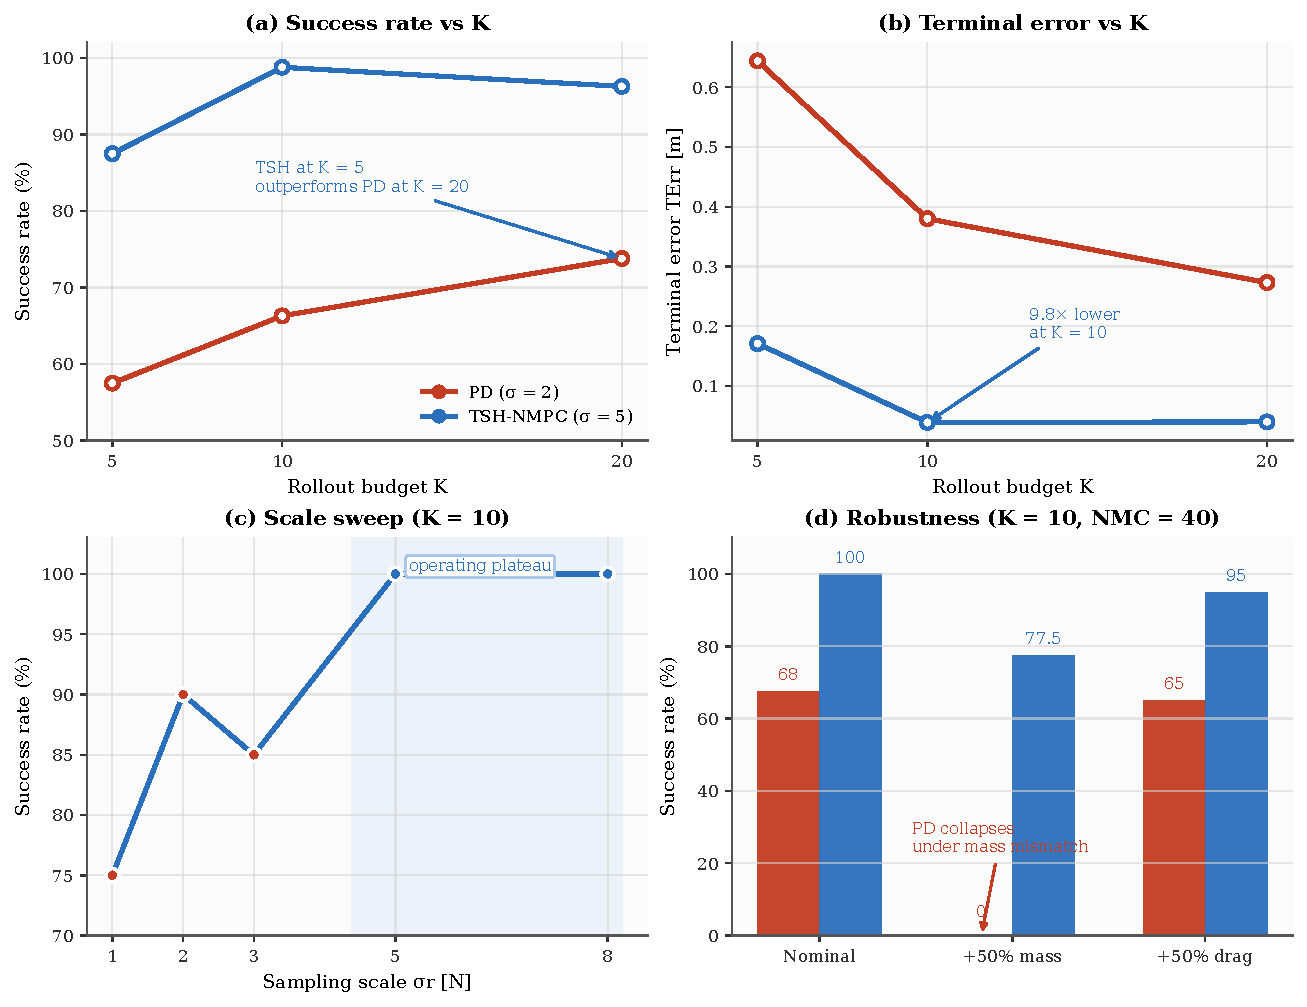
\includegraphics[width=\textwidth]{experiments/results_v6/fig2_quant.pdf}
\caption{Main quantitative evidence on \textsc{narrow}.
(a,b) Success rate and terminal error versus $K$: TSH-NMPC
outperforms PD across budgets. (c) $\sigma_r$ sweep ($K{=}10$):
success saturates at $\sigma_r \ge 5$ N, defining the operating
plateau (shaded). (d) Robustness under $+50\%$ mass and $+50\%$
drag: TSH-NMPC retains success while PD collapses under mass
mismatch.}
\label{fig:quant}
\end{figure}

On \textsc{two\_gate} and \textsc{u\_shape} ($K = 10$, $\Nm = 40$),
PD achieves $100\%$ success; $R_{1,\sigma=5}$ matches $40/40$ and
strictly improves $\TErr$ and $\IAE$ (Supplementary Table~S1).
\phantomsection\label{sec:exp-sigma-sweep}

The $\sigma_r$ sweep in Fig.~\ref{fig:quant}(c) shows that
$\sigma_r \le 1\,\mathrm{N}$ is too tight, $\sigma_r = 2$--$3\,\mathrm{N}$
improves but does not saturate success, and $\sigma_r \ge
5\,\mathrm{N}$ forms the operating plateau (full table with CIs
in Supplementary Table~S6).\phantomsection\label{tab:sigma-sweep}\phantomsection\label{sec:exp-crossconfig}

Under $+50\%$ mass, PD collapsed to $0/40$ while TSH-NMPC retained
$31/40$ success at $K = 10$; across three seeds this rose to
$99/120$ vs.\ $0/120$. Under $+50\%$ drag, success improved from
$26/40$ to $38/40$ (full tables in Supplementary Tables~S2--S3).

\subsubsection{PI-PD, Single-Source-Wide Ablation, and MPPI/CEM Baselines}\label{sec:exp-pi-baseline}

Additional ablations ruled out simpler alternatives. PI-PD also
failed under $+50\%$ mass. $R_{0,\sigma=5}$ was statistically
equivalent to $R_{1,\sigma=5}$ ($p = 0.508$). MPPI and CEM required
wider sampling or larger budgets to match success, and accepted worse
terminal tracking. Full PI-PD, MPPI, CEM, and iCEM sweeps are in
Supplementary Tables~S7--S8.
\phantomsection\label{sec:exp-r0-pd-s5}\phantomsection\label{sec:exp-mppi-cem}

\subsection{Diversity-over-Accuracy Ablation: Learned Prior as Source B}\label{sec:exp-negabl}

Can Source~B be improved by a \emph{learned predictor}? $A_{3}$ keeps
Source~A unchanged ($K_A = K/2$ PD-centred Gaussian) but draws
$K_B = K/2$ from a $27{,}935$-parameter TRM trained on $50{,}000$
closed-loop PD+CBF trajectories; otherwise identical to TSH-NMPC.

\textbf{Headline ($\Nm = 300$).} The well-powered comparison
($\Delta_{\min} \approx 0.06$) is decisive: $R_{1,\sigma=5}$
($293/300$, $97.7\%$) and $R_{0,\sigma=5}$ ($296/300$, $98.7\%$)
dominate $A_3$ ($266/300$, $88.7\%$; McNemar $p = 7.4 \times 10^{-6}$).
In this benchmark, random wide sampling outperformed the learned
source, indicating that candidate diversity was more important than
single-step prediction accuracy. A second TRM with better one-step
accuracy performed worse, consistent with diversity collapse
(Supplementary Table~S9).

\subsection{Comparison against CasADi+IPOPT NLP-based NMPC}\label{sec:exp-casadi}

We evaluate multiple-shooting NMPC with CasADi+IPOPT~\cite{AND19,WAC06}
(identical $Q,R$, soft obstacle penalty; details are provided in Supplementary Sec.\,S4).
CasADi-$H20$ achieved $80/80$ success on nominal \textsc{narrow}
with $\TErr = 0.003\,\mathrm{m}$ and $5.3\,\mathrm{ms}$ mean
latency. TSH-NMPC achieved the same success rate at $K \ge 20$
($\TErr = 0.032\,\mathrm{m}$ at $K{=}20$, $0.015\,\mathrm{m}$ at
$K{=}50$) but did not match CasADi's terminal accuracy. Under
$+50\%$ mass, TSH-NMPC at $K = 150$ reached $40/40$ versus
CasADi's $37/40$. The key distinction is fixed rollout computation
instead of data-dependent NLP iterations. Per-call controller cost
is $5.7\,\mathrm{ms}$ at $K = 10$, close to CasADi's
$5.3\,\mathrm{ms}$; full per-step latency including simulator
bookkeeping is $10.7 \pm 2.1\,\mathrm{ms}$. P99, deadline overruns,
and McNemar details are in Supplementary Tables~S10--S11.
TSH-NMPC should therefore be interpreted as a fixed-budget solver-free
alternative, not as a higher-accuracy replacement for NLP-based
NMPC.\phantomsection\label{tab:casadi}\phantomsection\label{sec:exp-fallback}\phantomsection\label{sec:exp-latency}

\begin{figure}[t]
\centering
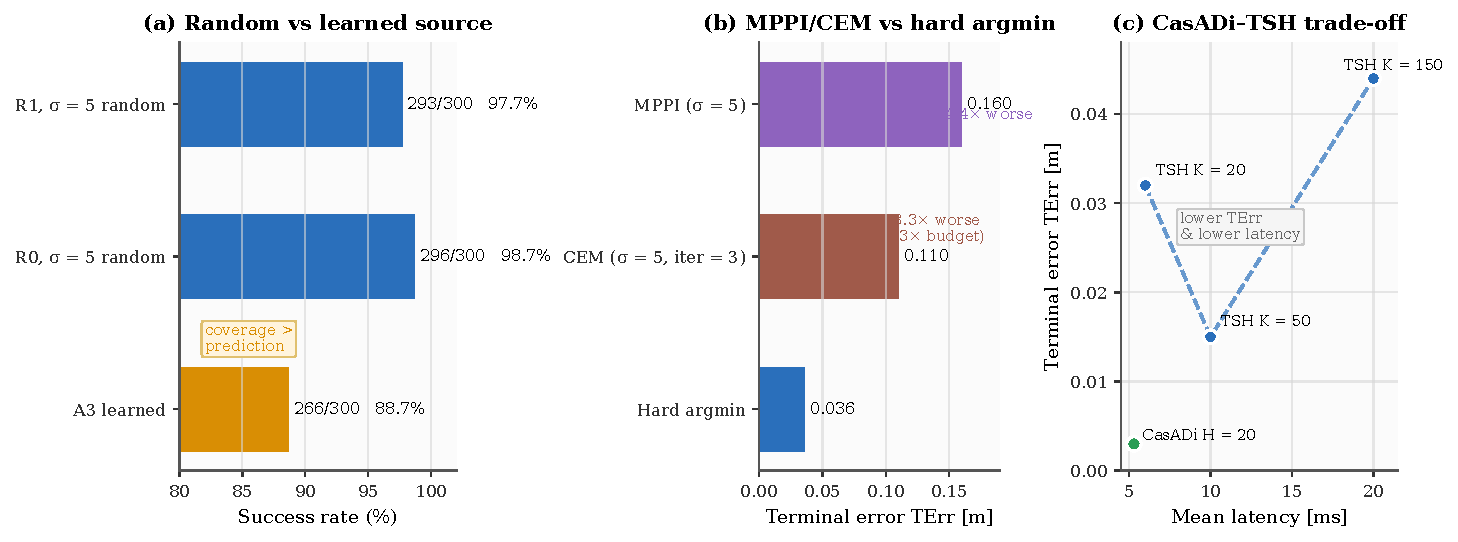
\includegraphics[width=\textwidth]{experiments/results_v6/fig3_comparisons.pdf}
\caption{Controlled comparisons. (a) Random wide vs.\ learned source
($\Nm = 300$): coverage dominates prediction accuracy.
(b) MPPI/CEM vs.\ hard-argmin: soft weighting and refitting degrade
terminal tracking. (c) CasADi vs.\ TSH latency--error trade-off:
lower $\TErr$ and latency for CasADi; fixed-budget computation for
TSH.}
\label{fig:comparisons}
\end{figure}

%====================================================================
\section{Discussion}\label{sec:discussion}
%====================================================================

\subsection{Mechanism and Relation to Alternatives}\label{sec:disc-mechanism}

What the ablation shows is that the three pieces have separate jobs.
Wider sampling ($\sigma \ge 5$) is what makes escape candidates
possible. Hard-argmin keeps those rare escape candidates from getting
washed out by soft averaging ($4.4\times$ lower $\TErr$ than MPPI
at matched $\sigma$). The CBF projection stops collisions that wider
exploration would otherwise cause. The three pieces only work
together in this narrow-passage regime: if the sampling is narrow
you cannot escape, soft aggregation dilutes escape candidates, and
without the safety filter wide exploration is unsafe.

At matched $\sigma = 5$, hard-argmin gave lower terminal error than
MPPI ($4.4\times$ worse $\TErr$) and CEM ($3.3\times$ worse $\TErr$
at $3\times$ the rollout budget). Against CasADi+IPOPT, the method
trades terminal accuracy for a fixed-budget computation.

\subsection{Limitations and Future Work}\label{sec:limitations}

A few limits narrow how far the results carry:
(i)~simulation only; hardware would need to deal with attitude lag
and non-isotropic disturbances; (ii)~single 6D quadrotor model;
(iii)~author-constructed benchmarks; (iv)~$\sigma_r$ is a fixed
scalar, not yet adaptive; (v)~the diversity-over-accuracy finding
is tied to roughly isotropic escape geometries;
(vi)~Proposition~\ref{prop:mono} gives monotone expected cost only,
with no violation-probability bound. Stress tests with Dryden wind
and dynamic obstacles are reported in the supplementary material; the
remaining gap is hardware validation including attitude lag, actuator
limits, sensing noise, and PX4 SITL deployment.


\section{Conclusion}\label{sec:conclusion}

This paper looked at a specific way that PD-centred sampling NMPC
can break down in narrow-passage quadrotor flight. When the PD
nominal points toward a conservative barrier boundary, narrow
sampling may give no control that actually goes through the gap.
TSH-NMPC fixes this by putting together three things: wide
PD-centred sampling, hard-argmin rollout selection, and DT-CBF
projection. The experiments show these three pieces each deal with
a different piece of the failure: one generates escape candidates,
one keeps the rare useful ones, and one filters out collisions. In
the end, the controller is best thought of as a solver-free,
fixed-budget option for this benchmark setting. It gets to the same
success rate as NLP-based NMPC on the tasks tested, but it does not
match the terminal accuracy. The results are still only from
simulation and use a fixed sampling scale; hardware tests and
adaptive scale selection still need to be done.

\begin{thebibliography}{99}

\bibitem{AME17}
A.~D. Ames, X.~Xu, J.~W. Grizzle, and P.~Tabuada, ``Control barrier
function based quadratic programs for safety critical systems,''
\emph{IEEE Trans.\ Autom.\ Control}, vol.~62, no.~8, pp.~3861--3876,
Aug.\ 2017.

\bibitem{BOT13}
Z.~I. Botev, D.~P. Kroese, R.~Y. Rubinstein, and P.~L'Ecuyer, ``The
Cross-Entropy Method for Optimization,'' in \emph{Handbook of
Statistics}, vol.~31, ch.~3, 2013.

\bibitem{GAN21}
M.~S.~Gandhi, B.~Vlahov, J.~Gibson, G.~Williams, and
E.~A.~Theodorou, ``Robust model predictive path integral control:
Analysis and performance guarantees,'' \emph{IEEE Robot.\ Automat.\
Lett.}, vol.~6, no.~2, pp.~1423--1430, Apr.\ 2021.

\bibitem{HOL79}
S.~Holm, ``A simple sequentially rejective multiple test procedure,''
\emph{Scand.\ J.\ Stat.}, vol.~6, no.~2, pp.~65--70, 1979.

\bibitem{JAN22}
M.~Janner \emph{et al.}, ``Planning with diffusion for flexible
behavior synthesis,'' \emph{ICML}, 2022.

\bibitem{KAH18}
G.~Kahn, A.~Villaflor, B.~Ding, P.~Abbeel, and S.~Levine,
``Self-supervised deep RL with generalized computation graphs for
robot navigation,'' \emph{ICRA}, 2018.

\bibitem{SUN22}
S.~Sun, A.~Romero, P.~Fojt, G.~Cioffi, and D.~Scaramuzza, ``A
comparative study of nonlinear MPC and differential-flatness-based
control for quadrotor agile flight,'' \emph{IEEE Trans.\ Robot.},
vol.~38, no.~6, pp.~3357--3373, Dec.\ 2022.

\bibitem{PAN17}
Y.~Pan, C.-A. Cheng, K.~Saigol, K.~Lee, X.~Yan, E.~Theodorou, and
B.~Boots, ``Agile autonomous driving using end-to-end deep imitation
learning,'' \emph{RSS}, 2017.

\bibitem{RUB04}
R.~Y. Rubinstein and D.~P. Kroese, \emph{The Cross-Entropy Method: A
Unified Approach to Combinatorial Optimization, Monte-Carlo
Simulation, and Machine Learning.}\ Springer, 2004.

\bibitem{WAN17}
L.~Wang, A.~D. Ames, and M.~Egerstedt, ``Safety barrier certificates
for collisions-free multirobot systems,'' \emph{IEEE Trans.\ Robot.},
vol.~33, no.~3, pp.~661--674, Jun.\ 2017.

\bibitem{WIL17}
G.~Williams, N.~Wagener, B.~Goldfain, P.~Drews, J.~M.~Rehg,
B.~Boots, and E.~A.~Theodorou, ``Information theoretic MPC for
model-based reinforcement learning,'' in \emph{Proc.\ IEEE Int.\ Conf.\
Robot.\ Autom.\ (ICRA)}, 2017, pp.~1714--1721.

\bibitem{WIL18}
G.~Williams, P.~Drews, B.~Goldfain, J.~M.~Rehg, and
E.~A.~Theodorou, ``Information-theoretic model predictive control:
Theory and applications to autonomous driving,'' \emph{IEEE Trans.\
Robot.}, vol.~34, no.~6, pp.~1603--1622, Dec.\ 2018.

\bibitem{OKA20}
M.~Okada, L.~Martinez, and T.~Taniguchi, ``Variational inference MPC
for multi-modal control proposals,'' \emph{IEEE Robot.\ Automat.\
Lett.}, vol.~5, no.~4, pp.~5580--5587, 2020.

\bibitem{AND19}
J.~A.~E. Andersson, J.~Gillis, G.~Horn, J.~B. Rawlings, and M.~Diehl,
``CasADi: A software framework for nonlinear optimisation and
optimal control,'' \emph{Mathematical Programming Computation},
vol.~11, no.~1, pp.~1--36, 2019.

\bibitem{WAC06}
A.~W{\"a}chter and L.~T. Biegler, ``On the implementation of an
interior-point filter line-search algorithm for large-scale nonlinear
programming,'' \emph{Mathematical Programming}, vol.~106, no.~1,
pp.~25--57, 2006.

\bibitem{CAM08}
M.~C. Campi and S.~Garatti, ``The exact feasibility of randomized
solutions of uncertain convex programs,'' \emph{SIAM J.\ Optim.},
vol.~19, no.~3, pp.~1211--1230, 2008.

\bibitem{CAM18}
M.~C. Campi and S.~Garatti, ``Wait-and-judge scenario optimisation,''
\emph{Mathematical Programming}, vol.~167, no.~2, pp.~307--346, 2018.



\end{thebibliography}

% Supplementary material containing MPPI/CEM temperature sweep tables,
% full negative-ablation tables, CasADi NLP methodology details,
% CBF fallback full table, robustness details, latency details,
% and multiple-comparison correction details is available at:
% https://github.com/VickylastShao/CBF-Projected-Hard-Argmin-Sampling-for-Safe-Quadrotor-Navigation

\end{document}
